\documentclass[12pt]{scrartcl}
\usepackage[ngerman]{babel}


\usepackage{amsmath, amssymb}

\usepackage{array}  % for the tables

\usepackage{nameref}  % for referencing with name

\usepackage{hyperref}  % for hyperlinks

\usepackage{mathrsfs}

\usepackage{graphicx}  % for the images

\usepackage{glossaries}

\usepackage{xcolor, colortbl}

\usepackage{gensymb} % for \degree

\usepackage{pgfplots}

\usetikzlibrary{arrows}

% \usepgfplotslibrary{external}

% \tikzexternalize

\definecolor{Gray}{gray}{0.85}

% hyperlinks
\hypersetup{
    colorlinks,
    citecolor=black,
    filecolor=black,
    linkcolor=black,
    urlcolor=black
}

\bibliographystyle{IEEetran}




\author{David Jäggli}

\title{Analysis übergreifende Themen}



% ---------- Begin Main Document ----------- %



\begin{document}

\maketitle

\tableofcontents

\section{Zusammenfassende Tabelle}
\begin{center}
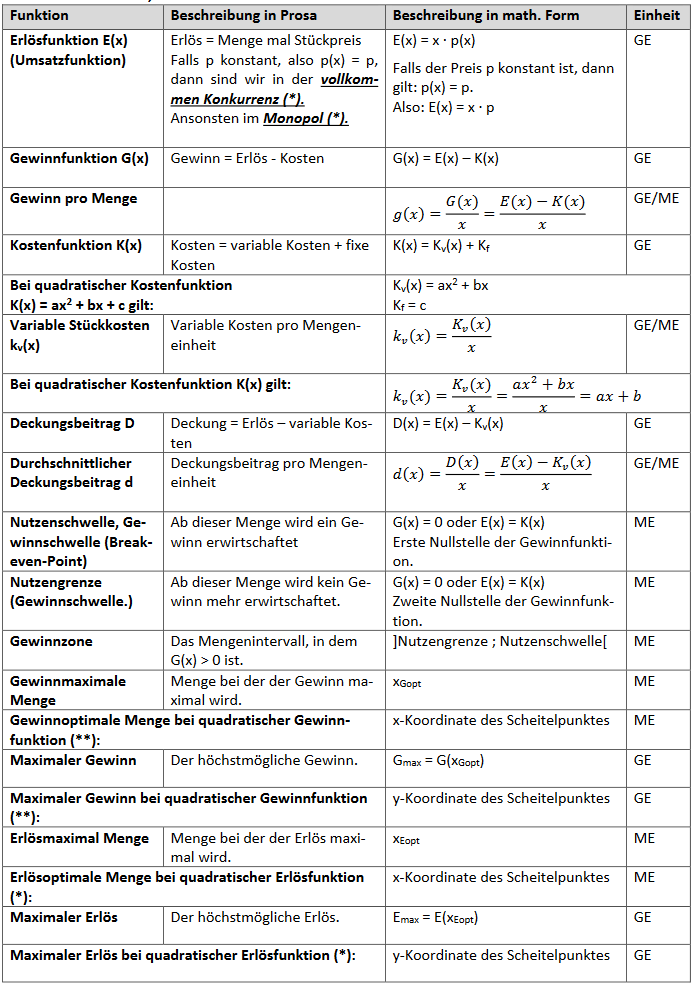
\includegraphics[width=16cm]{img/Wirtschaftstabeue-math.png}
\end{center}

\newpage
\section{Allgemeine Formeln}
\subsection{Volumen}
Kugel: $\frac{4}{3} \cdot r^3 \pi$ \\
Kegel: $\frac{1}{3}G \cdot h = \frac{1}{3} \pi r^2 \cdot h$

\subsection{Fläche}
Kreis: $r^2 \pi $\\
Dreieck: $g \cdot h$\\
Paralellogram: $\frac{g1 + g2}{2} \cdot h$


\newpage
\section{Trigonometrie}

\begin{center}
    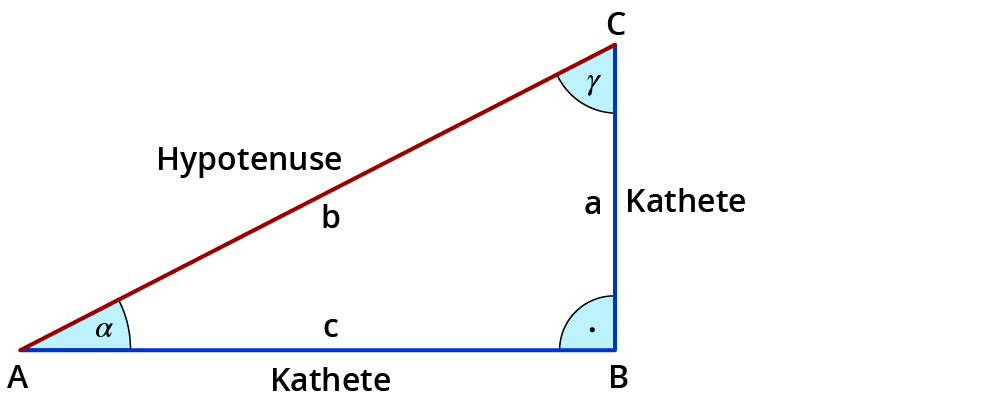
\includegraphics[width=13cm]{img/rechtw_dreieck.png}\\
\end{center}

\noindent
<<<<<<< HEAD:ANLS/Allg/main.tex
% Anwendungsbeispiel Strassensteigung:\\
% Wobei in diesem Fall Höhe = Gegenkathete (GK) und Breite = Ankathete (AK) gilt.\\
% Steigung = $\cfrac{Hoehe}{Breite}$
% \hspace{0pt}\\
% \hspace{0pt}\\
% Das Gleiche kann mit dem Winkel $\alpha$ und Tangens berechnet werden.
% Steigung (resp. Verhältnis von Höhe zu Breite) = $tan(\alpha) \Rightarrow \alpha = \arctan\left(\cfrac{GK}{AK}\right)$

\noindent
AK = Ankathete (hier c von $\alpha$)\\
GK = Gegenkathete (hier a von $\alpha$)\\
=======
AK = Ankathete (hier von $\alpha$)\\
GK = Gegenkathete (hier von $\alpha$)\\
>>>>>>> 4fc882b843b46055b13cf9c4362bb0a7e579e3bb:SEM1/ANLS/Allg/main.tex

\subsection{Tangens}
Der Tangens ist eine ungerade Funktion $\rightarrow tan(-\alpha) = -tan(\alpha)$\\
\hspace{0pt}\\
\noindent
$tan(\alpha) = \cfrac{\text{GK}}{\text{AK}} = \cfrac{sin(\alpha)}{cos(\alpha)}$\\
\hspace{0pt}\\
\hspace{0pt}\\
$\alpha = tan^{-1}\left(\cfrac{\text{GK}}{\text{AK}}\right)$
\hspace{0pt}\\
\hspace{0pt}\\

\noindent
\textbf{Wichtige Tangenswerte:}
\renewcommand{\arraystretch}{2.5}
\begin{center}
    \begin{tabular}{ | m{6em} | m{5em} | m{5em} | m{5em} | m{5em} | m{5em} |}
        \hline
        Winkel & 0\degree & 30\degree & 45\degree & 60\degree & 90\degree \\ 
        \hline
        Tangenswert & 0 & $\cfrac{\sqrt{3}}{3}$ & 1 & $\sqrt{3}$ & undefined \\ 
        \hline
    \end{tabular}
\end{center}

\newpage

\section{Funktionen}
\subsection{Allgemein}
\subsubsection{Schnittpunkte}
\begin{itemize}
    \item Die Nullstellen einer Funktion sind die Werte $x_i$, für welche $f(x_i) = 0$ gilt.
    \item Der Schnittpunkt mit der y-Achse ist der Punkt $S(0; f(0))$.
\end{itemize}

\subsubsection{Symmetrien}

\begin{itemize}
    \item Eine Funktion heisst gerade, wenn $f(x) = f(-x)$ gilt. (Bsp. $f(x) = x^2$)
    \item Eine Funktion heisst ungerade, wenn $f(x) = -f(-x)$ gilt. (Bsp. $f(x) = x^3$)
\end{itemize}

\subsubsection{Abschnittsweise definierte Funktionen}

\[ y = g(x) = 
    \begin{cases} 
    \frac{1}{2}x    & x \in ]-\infty; -2] \\
    -2x+3           & x \in ]-2; 3]\\
    5               & x \in ]3;\infty[
 \end{cases}
\]

% \begin{tikzpicture}[line cap=round,line join=round,>=triangle 45,x=0.5cm,y=0.25cm]
%     \begin{axis}[
%     x=0.75cm,y=0.5cm, % size of the grid
%     axis lines=middle,
%     ymajorgrids=true,
%     xmajorgrids=true,
%     xmin=-10,
%     xmax=10,
%     ymin=-10,
%     ymax=10,
%     xtick={-11,-10,...,10},
%     ytick={-10,-9,...,9},]
%     \draw[line width=2pt,color=blue] (-10,-5) -- (-2,-1);
%     \begin{scriptsize}
%         \draw[color=blue] (-9.866,-4.728) node {$g$};
%         \draw[color=blue] (-1.906,7.172) node {$f$};
%         \draw[color=blue] (3.134,5.232) node {$h$};
%     \end{scriptsize}
% \end{axis}
% \end{tikzpicture}

\begin{center}
    \begin{tikzpicture}[line cap=round,line join=round,>=triangle 45,x=1cm,y=1cm]
        \begin{axis}[
            x=0.75cm,
            y=0.35cm,
            xmin=-10, xmax=10,
            ymin=-10, ymax=10,
            xtick={-10,-8, ..., 10},
            ytick={-10,-8, ..., 10},
            grid=both,
        ]

        \draw (0, 50) -- (80, 90);
        \draw (80, 170) -- (130, 70);
        \draw (130, 150) -- (200, 150);
            % \addplot [
            % domain=-10:10, 
            % samples=100, 
            % color=red,
            % ]
            % {x^2 - 2*x - 1};    
        \end{axis}
    \end{tikzpicture}
\end{center}



% \bibliography{quantum_ready}

\end{document}